%%%%%%%%%%%%%%%%%%%%%%%%%%%%%%%%%%%%%%%%%
% Short Sectioned Assignment
% LaTeX Template
% Version 1.0 (5/5/12)
%
% This template has been downloaded from:
% http://www.LaTeXTemplates.com
%
% Original author:
% Frits Wenneker (http://www.howtotex.com)
%
% License:
% CC BY-NC-SA 3.0 (http://creativecommons.org/licenses/by-nc-sa/3.0/)
%
%%%%%%%%%%%%%%%%%%%%%%%%%%%%%%%%%%%%%%%%%

%----------------------------------------------------------------------------------------
%	PACKAGES AND OTHER DOCUMENT CONFIGURATIONS
%----------------------------------------------------------------------------------------

\documentclass[paper=a4, fontsize=11pt]{scrartcl} % A4 paper and 11pt font size

\usepackage[T1]{fontenc} % Use 8-bit encoding that has 256 glyphs
% \usepackage{fourier} % Use the Adobe Utopia font for the document - comment this line to return to the LaTeX default
\usepackage[english]{babel} % English language/hyphenation
\usepackage{amsmath,amsfonts,amsthm} % Math packages
\usepackage{siunitx}
\usepackage{mathtools} %for delimiters
\usepackage{braket}
\usepackage{gensymb}
\usepackage{natbib}
\bibliographystyle{apalike}

% for bibliography compatibility
\DeclareOldFontCommand{\rm}{\normalfont\rmfamily}{\mathrm}
\DeclareOldFontCommand{\sf}{\normalfont\sffamily}{\mathsf}
\DeclareOldFontCommand{\tt}{\normalfont\ttfamily}{\mathtt}
\DeclareOldFontCommand{\bf}{\normalfont\bfseries}{\mathbf}
\DeclareOldFontCommand{\it}{\normalfont\itshape}{\mathit}
\DeclareOldFontCommand{\sl}{\normalfont\slshape}{\@nomath\sl}
\DeclareOldFontCommand{\sc}{\normalfont\scshape}{\@nomath\sc}
\DeclareRobustCommand*\cal{\@fontswitch\relax\mathcal}
\DeclareRobustCommand*\mit{\@fontswitch\relax\mathnormal}

\DeclarePairedDelimiter\abs{\lvert}{\rvert}%
\DeclarePairedDelimiter\norm{\lVert}{\rVert}%
% Swap the definition of \abs* and \norm*, so that \abs
% and \norm resizes the size of the brackets, and the
% starred version does not.
\makeatletter
\let\oldabs\abs
\def\abs{\@ifstar{\oldabs}{\oldabs*}}
%
\let\oldnorm\norm
\def\norm{\@ifstar{\oldnorm}{\oldnorm*}}
\makeatother

\sisetup{
    %output-decimal-marker={,}% just uncomment if you want to use comma as the decimal marker!
}

\usepackage{sectsty} % Allows customizing section commands
\allsectionsfont{\centering \normalfont\scshape} % Make all sections centered, the default font and small caps

\usepackage{fancyhdr} % Custom headers and footers

\usepackage[toc, nonumberlist]{glossaries} % Glossary, acronyms
\setacronymstyle{long-short}
\makenoidxglossaries

\pagestyle{fancyplain} % Makes all pages in the document conform to the custom headers and footers
\fancyhead{} % No page header - if you want one, create it in the same way as the footers below
\fancyfoot[L]{} % Empty left footer
\fancyfoot[C]{} % Empty center footer
\fancyfoot[R]{\thepage} % Page numbering for right footer
\renewcommand{\headrulewidth}{0pt} % Remove header underlines
\renewcommand{\footrulewidth}{0pt} % Remove footer underlines
\setlength{\headheight}{13.6pt} % Customize the height of the header

\numberwithin{equation}{section} % Number equations within sections (i.e. 1.1, 1.2, 2.1, 2.2 instead of 1, 2, 3, 4)
\numberwithin{figure}{section} % Number figures within sections (i.e. 1.1, 1.2, 2.1, 2.2 instead of 1, 2, 3, 4)
\numberwithin{table}{section} % Number tables within sections (i.e. 1.1, 1.2, 2.1, 2.2 instead of 1, 2, 3, 4)

% \setlength\parindent{0pt} % Removes all indentation from paragraphs - comment this line for an assignment with lots of text

\newcommand{\secstar}[1]{\addcontentsline{toc}{section}{#1}\section*{#1}}

%----------------------------------------------------------------------------------------
%	Glossary and bibliography
%----------------------------------------------------------------------------------------

\loadglsentries{glossary.tex}
\glsaddall

%----------------------------------------------------------------------------------------
%	TITLE SECTION
%----------------------------------------------------------------------------------------

\newcommand{\horrule}[1]{\rule{\linewidth}{#1}} % Create horizontal rule command with 1 argument of height

\title{
\normalfont \normalsize
\textsc{The Open University} \\ [25pt] % Your university, school and/or department name(s)
\horrule{0.5pt} \\[0.4cm] % Thin top horizontal rule
\huge A Critical evaluation of Quantum Key Distribution, focusing on SARG04 as a benchmark \\ % The assignment title
\horrule{2pt} \\[0.5cm] % Thick bottom horizontal rule
}

\author{William Ockmore} % Your name

\date{\normalsize\today} % Today's date or a custom date

\begin{document}

\maketitle % Print the title

%----------------------------------------------------------------------------------------
%	ABSTRACT
%----------------------------------------------------------------------------------------

\secstar{Abstract}
Quantum key distribution (QKD) allows two parties to share an unconditionally secure key by
means of a quantum channel, where eavesdropping can be detected in the signal itself.
In this critical literature review, two of the most prominent prepare and measure protocols are
described, with focus on their sifting phase. The limitations of these protocols are analysed,
centering on the Photon Number-Splitting (PNS) attack as an eavedropping method.
A more recent protocol, SARG04, is detailed, and its benefits and limitations relative to
these previous protocols are described at length, with particular focus on the comparison with BB84.
Within this analysis, it is found that BB84 with decoy states has a higher secret key rate and secure
distance, under realistic experimental parameter sets, than SARG04 with decoy states. This is the case
even in the scenario of two photon pulses, for which SARG04 was developed. The only exception
is the case of a channel with very low quantum bit error, and a multi-photon pulsed source,
with the expectation that SARG04 is used when Eve (an eavesdropper) is present.
\vfill
\textbf{(word count for abstract - 179)}

%----------------------------------------------------------------------------------------
%	CONTENTS
%----------------------------------------------------------------------------------------

\clearpage
\addcontentsline{toc}{section}{Contents}
\tableofcontents

%----------------------------------------------------------------------------------------
%	INTRODUCTION
%----------------------------------------------------------------------------------------
\clearpage
\section{Introduction}

Quantum key distribution (QKD) is the study of quantum mechanics
as a mechanism to share an unconditionally secure key between two parties. Since the first
protocol (BB84 or the four-state protocol) was proposed in the mid 1980s \citep{BB84},
the field has slowly grown; it now encompasses many different
protocols, using a variety of quantum processes to enable ever more secure
sharing of information. Still amongst the most widely
used, BB84 is one of the most straightforward; using two sets of two non-orthogonal basis states,
the key is encrypted in the state sent, and when the classical bit-sifting phase
takes place Alice (the sender) communicates to Bob (the receiver) the basis used for a selection
of the states sent. If the error is within the acceptable bounds, they can be sure that
their key is secure, and communicate the basis used for the rest of the states. In this
way, the unconditional security is achieved.

One major problem with BB84 is its reliance on a single photon source for unconditional security.
Eve (the eavesdropper) has no restrictions other than the laws of physics. If the source used to send the key sends two or more quantum
states per bit, Eve can execute a Photon Number Splitting (PNS) attack; for every pulse of two or more photons,
she stores one state and lets the other state(s) continue on to Bob. Once Alice reads out the bases she used, Eve
will therefore have the complete key without the knowledge of the other participants. This
can be generalised to all prepare and measure protocols.

The area of study for this report focuses on the use of a recent protocol, SARG04, as a means to improve the
robustness against PNS attacks. It compares its efficacy
to BB84 and others, and discusses the impact of decoy states and other practical methods to increase security.

The objectives for the report are as follows: to give a brief history of QKD and its possible impact on current
society; to discuss the limitations of historical protocols in the real world; to give a detailed analysis of the
SARG04 protocol and its benefits over previous protocols; and finally to outline possible improvements,
either through practical engineering or new theory.

The search methodology used in this report involved first doing a broad search of academic articles, using google scholar and similar
tools, and then narrowing the scope through progressively more specific boolean search terms; then using papers already found to aid understanding
of the research area, and to provide other papers to study in the form of references.

%----------------------------------------------------------------------------------------
%	Classic protocols
%----------------------------------------------------------------------------------------
\clearpage
\section{The BB84 and B92 prepare and measure protocols}

In this chapter, we give a description of two QKD protocols; BB84 and B92.
They both belong to the family of \textit{prepare and measure} protocols, which
involve sending individual quantum states (qubits) down a quantum channel,
to be measured by a receiver at the other end.

\subsection{BB84}

BB84 was the first proposed QKD protocol \citep{BB84, historyBrassard}.

\subsubsection*{The protocol}
In BB84, Alice uses a single photon source to transmit a set of polarization states to Bob.
Both Alice and Bob agree to align
their polarizers in either the vertical/horizontal ($+$) basis, or the
complementary basis of $\pm 45 \degree$  ($\times$). Alice then transmits her set
down the quantum channel, randomly choosing one of the two bases for each
photon, whilst Bob measures in his choice of basis for each photon received.

\begin{center}
\begin{tabular}{c c c}
	$\ket{H}$  & codes for & $0_+$ \\
	$\ket{V}$  & codes for & $1_+$ \\
	$\ket{+45}$  & codes for & $0_\times$ \\
	$\ket{-45}$  & codes for & $1_\times$ \\
\end{tabular}
\end{center}

Both Alice and Bob now have a list of sent or received bits, each with a basis. The second
phase of the protocol is the classical sifting step: over the unsecured classical channel, they
first start by comparing which bases were used for each bit, and discarding the bits for which
they used different bases. For a list of size $N$ this step will on average reduce its size by half,
to $N/2$. Having matched the measurement basis, this list is referred to as the \textit{raw key} \citep{gisin2002}.

Alice and Bob now reveal a random sample of their raw key to one another, to compare for errors. By
comparing each bit publicly over the classical channel, they can estimate the error rate for
the quantum channel. If no errors are found, the raw key is already the secret key. If there are
errors, Alice and Bob must either correct for them or discard their key \citep{reviewScariani}. Both these actions can
take place over the classical channel; hence this step is called the \textit{classical post-processing}.
At the end of this phase, depending on how much information Eve could possess, Alice and Bob either share
a secret key, or they must discard the potentially compromised key.

\subsection{B92}
The B92 protocol, involving just 2 non-orthogonal states, is the
most minimalist QKD protocol in terms of encoding. Described by \citet{B92},
the B92 coding allows the receiver to learn whenever they get
the bit sent without further discussion from Alice.

\subsubsection*{The protocol}
B92 can be carried out using the two bases used in BB84. Following on from the above description, Alice sends either
$\ket{H}$ or $\ket{+45}$, and Bob chooses to measure the incoming bit in either the ($\times$) or the ($+$)
basis. Both of these states code for 0 in BB84; if Bob measures the state that codes for 1 ($\ket{-45}$ or
$\ket{V}$ respectively) he can be certain that Alice transmitted her bit in the opposite basis. Hence, B92
allows the participants to restrict their transmissions in the sifting phase to whether or not Bob made
a conclusive measurement for each bit sent. After discarding all bits for which Bob cannot be certain, the raw
key they are left with is on average $N/4$ bits long, for an initial transmission of $N$ bits \citep{B92}.

After a simple comparison of raw key length to the length of the initial string sent by Alice for the classical
post processing step, the participants either possess a secret key, or have been alerted to the possibility
of Eve's presence.

\subsection{Discussion}
Ultimate proofs exist for both protocols; a well known one for BB84
by \citet{proofBB84}; and similarly, for B92 there is \citet{tamakiProofB92}. Both rely on
conversion to EDP entanglement protocols; shortly after the first entanglement-based QKD protocol was
described by \citet{E91}, prepare-and-measure protocols were shown to have equivalent entanglement-based
versions by \citet{edpEquivProof}. It must be noted, however, that the above proofs are valid only
for perfect single photon sources.

Although sometimes easier to implement than the more popular BB84, it is more difficult to establish
unconditional security of B92, as it is much more sensitive to losses and noise in the
quantum channel. In the original paper, it is shown to be necessary
to rely on a strong reference pulse to guard against
losses and noise; again the security of this implementation has been proven
\citep{tamakiStrongRefProofB92}.

If perfect single photon sources were easily available,
these protocols would provide complete security, with no extensions required.
However, this is not the case for practical applications of QKD;
as discussed in the following chapter, real world limitations have a large impact.

%----------------------------------------------------------------------------------------
%	Limitations of the classical protocols
%----------------------------------------------------------------------------------------
\clearpage
\section{Limitations of QKD - Eavesdropping techniques}
In most literature on QKD, Eve is assumed, for the completeness of security proofs, to have no restrictions
on her eavesdropping, other than the fundamental limitations of quantum mechanics itself; namely, the
no-cloning theorem and the effects of measurement on a free particle. Briefly described here are two of the
most common eavesdropping techniques that are considered for BB84 and B92, followed by a more in-depth look
at classification of eavesdropping strategies and discussion of the relevant literature.

\subsection{Intecept-resend}
Potentially the most straightforward eavesdropping technique is the intercept-resend
strategy, which functions exactly the same for both BB84 and  B92.
Eve essentially takes the same actions as Bob; with her unrestricted capabilities, performs
a quantum nondemolition measurement on the incoming photons from Alice, measuring in either the $\times$
or the $+$ basis. If she has measured in the basis used by Alice, the photon continues on to Bob,
and Eve has obtained full information whilst introducing no errors to the signal. However, if she has measured
in the wrong basis, her result will be uncorrelated with Alice's; meanwhile, she will have sent along
a modified state, so even if Bob measures in the same basis as sent by Alice, half the time he will get the
wrong result \citep{reviewScariani}.


\subsection{Photon Number Splitting attack - PNS}
In real world applications of QKD, the photon source is never a true strong single photon emitter. Typically
a weak coherent pulse laser source is used \citep{satellites}.
These sources emit pulses of coherent states, often containing 2 or more photons.
This presents a problem for the security of BB84 and B92, as described below.

\subsubsection*{BB84}
The security weakness in coherent pulses comes from Eve's ability to nondestructively determine the number of photons
in a pulse. The principle of the PNS attack is that Eve will block all single photon pulses, and for any pulse where
multiple photons are detected, Eve will store in quantum memory a subset of the pulse, while allowing the rest to continue
on to Bob (through an ideal quantum channel, to ensure he receives the photons). During the sifting
phase, Alice and Bob's communications over the public channel can be used by Eve to construct
a complete key from the stored states. The major benefit to Eve with this method is that it does not introduce an error in the
states received by Bob; the only risk of detection comes from the losses due to single photon pulses being blocked \citep{kronberg2009}.

As long as these losses do not reach a critical threshold (dependent on the length of the communication channel and the expected losses),
Eve's actions remain undetected, and the security of the protocol is compromised.


\subsubsection*{B92}
Against B92, PNS attack is even more straightforward. No quantum memory is required; Eve performs
the same measurement as Bob, and blocks the message in the event of an inconclusive result \citep{kronberg2009}. The losses are attributed
to channel losses; as long as a critical threshold is not reached (as above), Eve will obtain full information of the key whilst remaining unnoticed.

\subsection{Classification of eavesdropping strategies and further discussion}
Strategies for eavesdropping on QKD protocols can be generally split into two main groups;
\textit{individual} and \textit{coherent}. Individual attacks involve
Eve probing each qubit individually as she recieves them; for coherent attacks
she may process multiple qubits at a time, and measure them \textit{coherently} \citep{gisin2002}.

\subsubsection*{Individual attacks}
Individual attacks impose a higher limitation on Eve, as she cannot wait for the sifting
phase before she takes her measurements - she must measure sequentially. Intercept-resend is classified as an individual attack.

In intercept-resend, after she has completed the process,
Eve is left with full information of half the bits in the full key ($I_E = 0.5$).
The measurement process introduces an error rate of 25\% (QBER $= Q = 0.25$)
into the key recieved by Bob. Using the assumptions given by \citet{csiszarAssump},
this means no secret key can be extracted. This is in fact true for \textit{all} protocols under an individual-type
attack \citep{reviewScariani}.

Even in the case where Eve does not eavesdrop on all photons in the key, and instead on just a fraction $p$,
then clearly $Q = p/4$ and

\begin{align}
I_E	= p/2 = 2Q
\end{align}

More errors in the received qubits can then be assumed in worst case to be an increase in Eve's information,
along with a corresponding decrease in Bob's information. When Eve's maximal information is compared with Bob's error
(given by his Shannon information), an inequality is recovered which describes the relative advantage of Bob or Eve.
The point at which this advantage shifts to Eve can be expressed as a specific error rate $Q_0$:

\begin{align}
	I(\alpha, \beta) = \mathrm{max} \left\{ I(\alpha, \epsilon) \right\}
	\quad
	\Leftrightarrow
	\quad
	Q = Q_0
	\approx 15\%
\end{align}

Hence a secure key can only be extracted if $Q \leq 15\%$. \citep{qber15proof, gisin2002, huttner1995}

\subsubsection*{Coherent attacks}
\citet{gisin2002} succintly summarises the work of \citet{proofBB84} and others
on the subject of coherent attacks; using two theorems, the upper bound is found for the QBER
of a protocol expected to withstand coherent attack.

The first theorem originates from the field of classical
cryptography \citep{csiszarAssump}; if Alice, Bob and Eve
at some point perform measurements on their quantum systems
they will obtain classical random variables $\alpha$, $\beta$
and $\epsilon$, respectively, with $P(\alpha, \beta, \epsilon)$ as the
joint probability distribution. The the necessary and sufficient condition
for Alice and Bob to extract a secret key is

\begin{align}
	I(\alpha, \beta) \geq I(\alpha, \epsilon)
	\qquad
	\mathrm{or}
	\qquad
	I(\alpha, \beta) \geq I(\beta, \epsilon)
\end{align}

Where $I(\alpha, \beta) = H(\alpha) - H(\alpha | \beta)$ denotes the mutual information,
and $H$ is the Shannon entropy.

The second theorem expresses Heisenberg's uncertainty relation in terms of available information
\citep{hall1995}: it sets a bound on the sum of information about Alice's key available to Bob
and Eve.

Let E and B be two observables in an $N$-dimensional
Hilbert space. Let $\epsilon$, $\beta$, $\ket{\epsilon}$ and $\ket{\beta}$ be the corresponding
eigenvalues and eigenvectors, respectively, and
let $c = \mathrm{max}_{\epsilon, \beta}\left\{\abs{\Braket{\epsilon|\beta}}\right\}$. Then

\begin{align}
	I(\alpha, \epsilon) + I(\alpha, \beta) \leq 2\mathrm{log}_2(Nc)
\end{align}

Where again, $I(\alpha, \epsilon) = H(\alpha) - H(\alpha | \epsilon)$ and
$I(\alpha, \beta) = H(\alpha) - H(\alpha | \beta)$ are the entropy differences
corresponding to the probability distribution of the eigenvalues $\alpha$ prior
to and deduced from and measurement by Eve and Bob, respectively.

Theorem 1 means that to generate a secure key, Bob must have more information than
Eve about the bits generated by Alice. Theorem 2 is a mathematical description of the
fact that if Eve performs some measurement providing her with information, then because of
the perturbation, Bob's information is necessarily limited.

Using symmetry arguments, and denoting the number of qubits received in the
correct basis by Bob as $n$, theorem two implies

\begin{align}
	I(\alpha, \epsilon) + I(\alpha, \beta) \leq n
\end{align}

Which simply means that the sum of Eve and Bob's information per qubit is
less than or equal to 1; they cannot collectively receive more information
than Alice sends out. Combined with theorem one, this leads to the result that
a secret key is obtainable whenever $I(\alpha, \beta) \geq n/2$.
Finally using $I(\alpha, \beta) = n\left[1-Q\mathrm{log}_2(Q) - (1-Q)\mathrm{log}_2(1-Q)\right]$,
the bound for $Q$ (the QBER) can be obtained:
\begin{align}
	Q\mathrm{log}_2(Q) + (1-Q)\mathrm{log}_2(1-Q) \leq 1/2
	\qquad
	\Rightarrow
	\qquad
	Q \leq 11\%
\end{align}

This bound, when arrived at this way in particular, is only valid in the case where the key is much longer than number of
qubits Eve attacks coherently - allowing the Shannon information used to represent averages over
many measurements which return classical, random variables. However, the full proof given by
\citet{proofBB84} can still be used even in the event of Eve coherently attacking an unlimited number
of qubits. Precisely the same bound of $11\%$ QBER is recovered.

\subsubsection*{Multi-photon pulses}
The two previous sections dealt with the classification of attacks Eve might perform. In summary, if Eve can only be
expected to perform individual attacks, then the threshold of QBER before a sifted key becomes insecure
(assuming an infinite, or finite but large raw key) is $15\%$; if she has unlimited capacity to coherently measure
the states sent over the quantum channel, then the upper bound is $11\%$. But what if Alice transmits to Bob
not single quantum states, but instead pulses of multiple states? This is the reality for practical QKD \citep{recentDecoy, huttner1995}.
Usually such weakly pulsed laser sources have low photon number $\mu$ per pulse; typically $\mu \ll 1$ \citep{reviewScariani}.

In this circumstance, Eve may perform the PNS attack described above; the effect on security can be large.
Remember that Eve is not restricted in the technology she uses; while all currently known transmission
mediums incur some loss over distance, Eve could replace the channel between Alice and Bob by a perfect
lossless channel, and with the extra power gained she is free to discard a certain proportion of pulses. Typical
attenuation values for optical fibre are on the order of $10^{-2} \si{\dB \km^{-1}}$; most research findings indicate that
under such conditions security can only be guaranteed over a medium distance; between 50 and $200\si{\km}$, depending on experimental
parameters and assumptions \citep{perf2protocols, satellites, experimentalComparison}.

But how realistic is a quantum nondemolition measurement, or a lossless channel?
Quantum nondemolition measurements have increasingly been the subject of research \citep{brassard2000};
ideal quantum nondemolition photon number measurements are beyond current technologies, although it may
be reasonable to assume that they are possible \citep{reviewScariani, nogues1999}.

For Eve to count photon number for a pulse, she must measure it without disturbing the degree of
freedom encoding the qubit. Eve must then store the qubit, in either a lossless looped
channel, or by mapping the qubit to quantum memory. This may be unrealistic;
as noted above, there is no perfect physical medium
for transmission, due to unavoidable Rayleigh scattering.
Attenuation of the qubits reduces her information, and Alice and Bob
may wait minutes before carrying out the sifting phase \citep{reviewScariani}; consequently, even if she chooses to
use the quantum memory, it must have close to unlimited decoherence time. Two possibilities left for Eve are suggested
by \citet{gisin2002}; either she must use high-fidelity, near lossless quantum teleportation of the qubits, or
she can convert the photons to another wavelength, without disturbing the qubit. In the forseeable future,
neither option is realistic; however advances in quantum and optical technologies may make PNS attacks a serious threat.


%----------------------------------------------------------------------------------------
%	SARG04
%----------------------------------------------------------------------------------------

\clearpage
\section{The SARG04 protocol}
In this chapter, the SARG04 protocol, first described in \citet{SARG04orig} is explained in the context of previously discussed protocols.
Its benefits and limitations are analysed, with reference to real world experiments and applications.

\subsection{Description of the protocol}
SARG04 as a protocol is very similar to BB84; in fact, the steps followed by Alice and Bob are identical until the classical sifting phase.
The same setup can be used in both cases, which makes comparison of the two protocols straightforward.

The same four states are used in SARG04 as in BB84; however rather than the state sent coding for the bit, the basis itself is used, as in B92.
After the raw key has been transmitted, Alice declares for each qubit one of four pairs of
non-orthogonal states $A_{\omega, \omega'} \left\{ \ket{\omega x}, \ket{\omega' z}\right\}$ with $\omega, \omega' \in \{ +, -\}$
and the convention that $\ket{\pm x}$ code for 0 and $\ket{\pm z}$ code for 1 \citep{SARG04orig}. Any two non-orthogonal bases $\sigma_x$
and $\sigma_z$ may be used; for example the + and $\times$ polarisation bases used in the earlier description of BB84 and B92. Within each set $A_{\omega, \omega'}$
the overlap of the two states is $\chi = \frac{1}{\sqrt{2}}$.

The procedure for extracting the bit values is outlined in the following example. Suppose Alice sends $\ket{-x}$ and declares $A_{- +}$.
If Bob has received this particular bit in the $\sigma_x$ basis, he will measure $\ket{-x}$ with certainty. He cannot be certain that Alice did
not send $\ket{+z}$ in this circumstance. However if he receives in the $\sigma_z$ basis, he will measure $\ket{-z}$ with probability $\frac{1}{2}$.
As this state is contradictory to the second member of the pair communicated by Alice, Bob knows that, in the absence of errors, Alice must have sent $\ket{-x}$.

\subsection{Benefits of SARG04}
As Alice does not communicate basis over the classical channel during the sifting phase, Eve does not have the ability to
unambiguously determine the measurement basis for a qubit. For all two-photon pulses she now cannot be certain of achieving
a valid result; for three photon pulses, she must implement an unambiguous state discrimination measurement $\mathcal{M}$, which succeeds with probability
$\frac{1}{2}$ \citep{branciardSARG04}. Hence in the case of two-photon pulses SARG04 is still provably secure, where BB84 is not \citep{perf2protocols}.

To attack SARG04 Eve may implement a specific version of the PNS attack; discarding all one- and two-photon pulses,
she performs $\mathcal{M}$, and with a conclusive result (occuring with probability $\frac{1}{2}$) she sends a new photon prepared in the good state to Bob.
This attack is referred to as \textit{intercept-resend with unambiguous discrimination attack} (IRUD) \citep{SARG04orig}. It needs neither the quantum memory or
the lossless channel, as the new state can be prepared at some location close to Bob. There is a critical channel attenuation $\delta_c$ at which IRUD is
always possible; for a conservative estimate of $\mu = 0.2$ as given in the original paper, $\delta_c = 25.6 \si{\dB} \approx 2\delta_c^{\mathrm{BB84}}$. Hence under
the circumstance of zero external QBER and incoherent attack, SARG04 gives twice the secure distance as BB84. This was independently verified by \citet{branciardSARG04}.
In their paper it was also shown that SARG04 has a higher secret key rate than BB84 under realistic source conditions and under the assumption of incoherent attack by Eve.
Their results for a Poisonnian attenuated laser source are shown in Figure 4.1.

\begin{figure}
	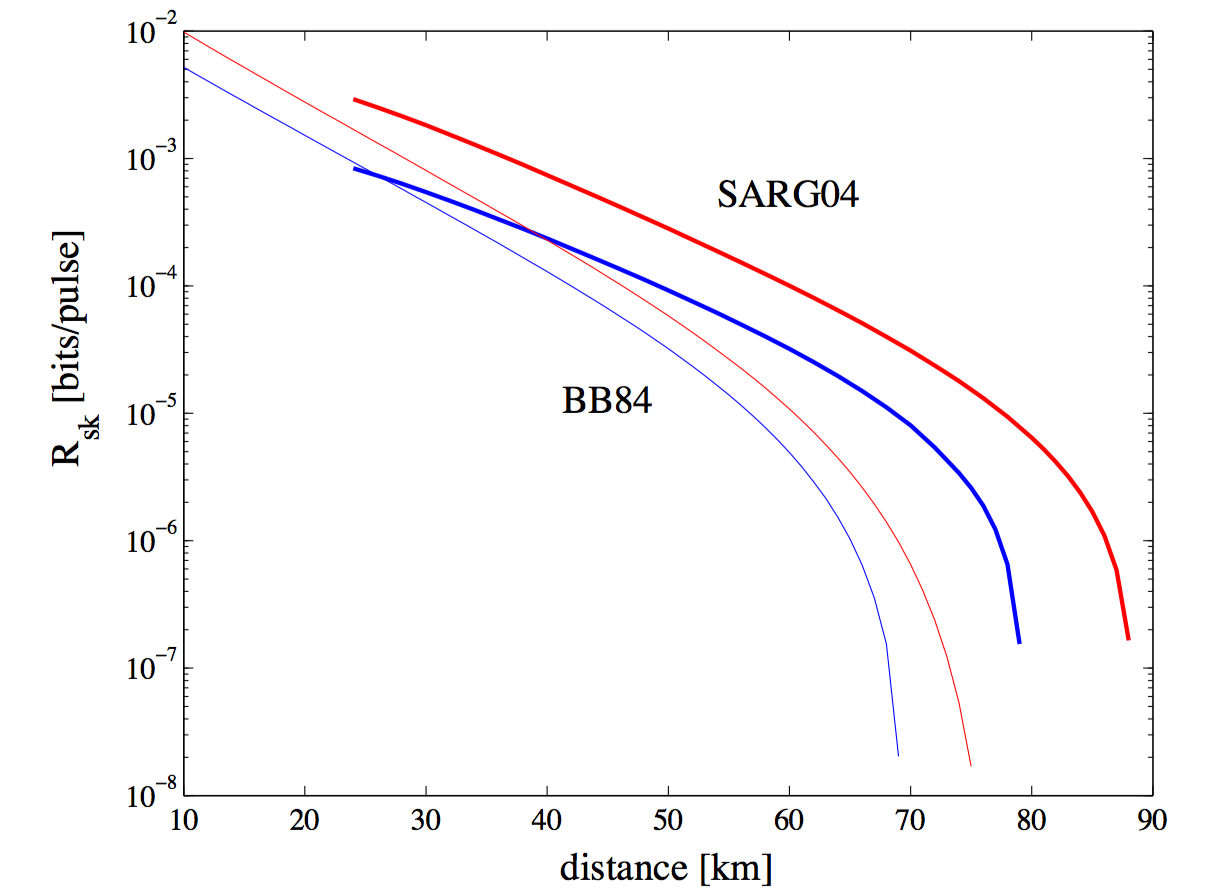
\includegraphics[width=\linewidth]{branciard-graph.png}
	\caption{Optimal $\mu$ and upper bound for secret key rate per pulse $R_{sk}$ with
	channel losses $\alpha=0.25\si{\dB \km^{-1}}$, detector quantum efficiency $\eta = 0.1$, dark count
	probability $p_d = 10^{-5}$, and channel visibility $V=$ 1, 0.95. The thick lines
	are results for SARG04, thin lines BB84. \citep{branciardSARG04}}
\end{figure}

\clearpage
\section{Limitations of SARG04}
\subsection{Single photon implementation}
In a single photon implementation, the upper bound on the attainable secret key rate is given by \citet{csiszarAssump} as

\begin{align}
r \leq R_{sk} = \max_{A \rightarrow A'}
\left\{
I(A':B) - I(A': E)
\right\}
\end{align}

where $A'$ represents any preprocessing performed by Alice, which gains a slight increase on the QBER bound where the secret key
becomes zero. This leads to the corresponding bounds for single photon SARG04 and BB84 as given in \citet{bounds, branciardSARG04}:

\bgroup
\def\arraystretch{1.2}% 1 is default, makes bigger spacing
\begin{center}
\begin{tabular}{c c c}
\hline
BB84 						& Lower & $Q \leq 12.4\%$ \\
\hphantom{BB84}	& Upper & $Q \geq 14.6\%$\\
\hline
SARG04  				& Lower & $Q \leq 10.95\%$ \\
\hphantom{BB84}	& Upper & $Q \geq 14.9\%$\\
\hline
\end{tabular}
\end{center}
\egroup

This does not take into account channel noise and subsequent reduction in visibility. In the case of a channel with
neligible dark count rate, the error rate on the sifted key is a function of the visibility. In the example of BB84, when
when the good basis is chosen the probabilities of a right or wrong measurement are $p_{\mathrm{right}} = \frac{1+V}{2}$ and
$p_{\mathrm{wrong}} = \frac{1-V}{2}$. This leads to

\begin{align}
	Q_{\mathrm{BB84}} =
	\frac{p_{\mathrm{wrong}}}{p_{\mathrm{right}} + p_{\mathrm{wrong}}}
	= \frac{1-V}{2}
\end{align}

As SARG04 codes by basis, whenever Bob accepts the good encoding basis (the one not used by Alice), he guesses right.
This is independent of the visibility so $p_{\mathrm{right}} = \frac{1}{2}$. If he chooses the wrong basis and accepts,
then this is due to error, and occurs with $p_{\mathrm{wrong}} = \frac{1-V}{2}$.

\begin{align}
	Q_{\mathrm{SARG04}} =
	\frac{p_{\mathrm{wrong}}}{p_{\mathrm{right}} + p_{\mathrm{wrong}}}
	= \frac{1-V}{2-V}
	\approx 1-V
\end{align}

Hence for a fixed visibility, the QBER is almost twice that of BB84 \citep{branciardSARG04}. Thus although the error bounds
are comparable, they are more restrictive for an implementation of SARG04 and the protocol is more sensitive to error in the channel.

\subsection{Key generation rate}
The nature of SARG04's sifting phase means that Bob may only accept on average $\frac{1}{4}$ bits. This is in contrast to BB84, where
choosing the correct measurement basis occurs 50\% of the time, hence Bob accepts $\frac{1}{2}$. The raw key generation rate for a general protocol,
under zero channel losses is

\begin{align}
R = \nu_s P_b
\end{align}

where $\nu_s$ is the repetition rate and $P_b$ is the probability that Bob accepts a bit. For a given source

\begin{align}
	R_{\mathrm{SARG04}} = \frac{\nu_s}{4} = \frac{R_{\mathrm{BB84}}}{2}
\end{align}

Under the same conditions, $\mu$ for SARG04 must then be twice that of BB84 for the same raw key rate \citep{perf2protocols, SARG04orig}.
In practical applications of the protocol this is a serious limitation; also, if Eve is not present then the use of SARG04 over BB84 is penalised
with no associated benefit.

As documented in \citet{experimentalComparison}, this leads (along with SARG04's sensitivity to channel visibility) to BB84 generating
more secret keys than SARG04 under real world conditions, where devices are imperfect and $V < 1$.

\subsection{Decoy states}
Decoy states were first proposed by \citet{decoyOrig} with one- and two-photon signals, with the more popular and realistic
intensity modulation implementation put forward soon after \citep{lo2005}.

\subsubsection*{Description of the technique}
The central idea behind decoy states is to randomly
change some tunable parameter $\xi$ in the protocol (most commonly the photon number/intensity $\mu$); using some subset
of possible values for the parameter to conduct the protocol itself, Alice and Bob then have a set of linear equations dependent
on the channel properties.

After transmitting the set of qubits, Alice reveals the list of values $\xi \in \chi$,
and after sorting the data Alice and Bob now have a linear system of $2\abs{\chi}$ equations

\begin{align}
R^\xi	= \sum_{n\geq0} R^\xi_n
\quad
\mathrm{and}
\quad
Q^\xi = \sum_{n\geq 0} \frac{R^\xi_n}{R^\xi}\epsilon_n
\end{align}

If Alice and Bob know the characteristics of their setup, they can determine with high confidence the expected
$R$ and $Q$ for a particular $\xi$; hence if Eve takes any action that will change either value substantially,
the participants can detect her presence. This greatly limits her options \citep{lo2005, reviewScariani}.

\subsubsection*{Optimum photon number}
In order to illustrate the benefits gained with decoy states, consider the concept of optimum $\mu$, a
variable that only becomes relevant beyond the discussion of ideal single-photon sources (as clearly,
the secret key rate $K$ scales linearly with $\mu$ in the case of a single photon source \citep{gisin2002}). % TODO: CITE
The probability for Alice's attenuated laser source to emit either one or two photons is given by

\begin{align}
	p_A(1) = \mu e^{-\mu}
	\quad
	\mathrm{and}
	\quad
	p_A(2) = \mu^2 e^{-\frac{\mu}{2}}
\end{align}

Obviously the ideal situation for security is for $p_A(2) \approx 0$; however this entails small $\mu$ and
by extension, small $R$. The optimum value for $\mu$ must maximise the achievable secret key rate.

Taking into account imperfect error correction, the definition for the secret key rate is given by

\begin{align}
	K = R\left[1-\operatorname{leak}_{EC}(Q) - I_E\right]
\end{align}

where $\operatorname{leak}_{EC}(Q)$ is the information loss due to imperfect error correction (so the leaked information
$\operatorname{leak}_{EC}(Q) \geq h(Q)$, with $h(Q)$ the binary Shannon entropy); and $I_E$ as usual is the maximal
information available to Eve \citep{reviewScariani}.

Rather than follow the lengthy derivation, results for optimal $\mu$ for an attenuated laser in the case without, and with,
decoy states are quoted below from \citet{reviewScariani}.

In the implementation without decoy states, the highest achievable secret key rate is
\begin{align}
	\frac{K}{\nu_s t t_B \eta}
	\approx
	\frac{1}{2}
	\mu_{\mathrm{opt}} F(Q)
	\qquad
	\text{(laser without decoy states)}
\end{align}
obtained for the optimal mean photon number
\begin{align}
	\mu_{\mathrm{opt}}
	\approx
	t t_B \eta
	\frac{F(Q)}{1-h(2Q)}
\end{align}
where $t$ is the transmittivity of the quantum channel, $t_B$ are the losses in Bob's
device, $\eta$ is the efficiency of the detector, and $F(Q) = 1 - h(2Q) - h(Q)$.

For the implementation with decoy states, the maximal value for $K$ is

\begin{align}
	\frac{K}{\nu_s t t_B \eta}
	\approx
	\frac{1}{2}
	\mu_{\mathrm{opt}}
	\left[1-2h(Q)\right]
	\qquad
	\text{(laser with decoy states)}
\end{align}
for optimal mean photon number
\begin{align}
	\mu_{\mathrm{opt}}
	\approx
	\frac{1}{2}
	\left[
	1 - \frac{h(Q)}{1-h(Q)}
	\right]
\end{align}

Consequently, without decoy states $\mu_{\mathrm{opt}} \propto t$, and hence
$K \propto t^2$: the larger the losses in the channel, the more attenuated the laser
must be. For guarding against PNS attacks, it must be ensured that Eve cannot reproduce
the detection rate at Bob's by using only photons from 2-photon pulses. With decoy states,
the fraction of detections that come from 2-photon pulses can be determined; if this fraction
is as low as is expected, a PNS attack can be ruled out. The major benefit gained is the recovery
of $K \propto t$ scaling. This is the same as for ideal single-photon sources \citep{lo2005, reviewScariani}.

\subsubsection*{Consequences for SARG04}

A comparison simulation of the performance of SARG04 and BB84 using decoy states was published by \citet{perf2protocols}. With the
addition of two way classical communications (allowing Alice and Bob to communicate with each other, rather than just
one-way) it was shown that for all realistic parameter sets, SARG04 had a smaller key generation rate and shorter secure
distance than BB84. In the case of small QBER, the optimum $\mu$ of SARG04 can be higher than BB84; this does not mean
however that the key generation rate is necessarily greater, as mentioned earlier. These results are in the case of general
attack by Eve.

It is interesting that the most robust and performant protocol is still BB84 (albeit with modifications such as the addition of
decoy states). In recent papers by \citet{recentDecoyBounds, recentDecoy}, the secret key rate was increased to almost $1\si{Mb \s^{-1}}$
over $50\si{km}$, with reduced sensitivity to finite-size effects; further legitimising real world applications of the protocol.
Even taking into account the most optimised decoy-state versions of SARG04, they still compare poorly to BB84 \citep{recentDecoySARG04}.

However the caveat that must be properly understood in these comparisons is that decoy states are a method to
gain knowledge on Eve's attack. If the attack is not taking place, then BB84 with its simpler sifting methodology
will produce a higher secret key rate; however, if an attack is taking place, then in two photon implementations
\textit{with small QBER}, SARG04 will generate a key with higher probability. In simple terms,
if BB84 can generate a key that is secure, it will do so faster; SARG04's application is for the times when this is
not possible \citep{perf2protocols, reviewScariani}.

\clearpage
\section{Conclusion}
In this review, SARG04 was introduced and compared to known prepare and measure protocols. It was found that although
it brings a novel way to foil a PNS attack by changing the classical communication phase of BB84, once other factors
of practical application - such as decoy states, key generation rate under imperfect conditions, and lossy channels -
are brought into account, it compares unfavourably to the original protocol in realistic scenarios.

Extensive analysis was taken on the classical protocols, attack vectors, and the direct limitations of SARG04. Possible improvements
to the methodology could include additional research into strong reference pulse based security and its implications for the protocol \citep{koashi2004};
as well as comparison to new protocols that have not yet been fully explored, such as KMB09 \citep{KMB09}.

The initial objectives given were considered before full understanding of the research area had been obtained. However
in terms of scope, the review has stayed reasonably close to the original outline. A brief history of QKD was given, although
its impact on society was not fully addressed. Limitations of historical protocols were investigated thoroughly; SARG04 was described
and its benefits and limitations discussed at length. The real world improvements possible were highlighted in the decoy state
method, although more was left to be said with regards to further study in the case of SARG04 itself.
\vfill
\textbf{total word count - 4602}


%------------------------------------------------


%----------------------------------------------------------------------------------------
\clearpage
\bibliography{bibliography.bib}

\clearpage
\printnoidxglossaries

\end{document}
